\chapter{Treiber}
\label{chap:Treiber}

\section{Treiber Architektur}
\subsection{Generelle Überlegungen}
\subsection{Anforderungen}
Der Treiber ist dafür verantwortlich Pakete aus Windows zu dem Server zu senden. Dabei müssen 3 Probleme gelöst werden:
\begin{itemize}
    \item Sammeln von IP Paketen aus Windows
    \item Verteilen von IP Paketen an Programme
    \item Kommunikation zwischen Treiber und Server
\end{itemize}
Außerdem sind müssen gewisse Standards von Performance, Stabilität und Ressourcen Intensität gehalten werden. Dabei haben wir versucht folgende Metriken einzuhalten:
\begin{itemize}
    \item Maximaler prozentuale CPU Auslastung von 3 %, bei einer 100 MB/s Übertragungsrate auf einem (Prozessor von Tests einsetzten)
    \item Maximaler Speicherverbrauch von 300 Mega Byte bei Verwendung von 2 übertragenen Netzwerkadaptern über eine Dauer von 30 Minuten.
    \item Wenn es zum Absturz des Treibers kommen sollte, darf das Betriebssystem nicht mit abstürzen.
    \item Der Treiber sollte weiter funktionieren, auch wenn während des Betriebs ein Netzwerkadapter ausfällt.
\end{itemize}
Zur Bedienungsfreundlichkeit wird eine CLI zur Verfügung gestellt mit welcher folgende Operationen ermöglicht werden:
\begin{itemize}
    \item Konfigurieren des Treibers über JSON, Key-Value Dateien oder über die Konsole
    \item Starten und Stoppen der Kommunikation des Treibers mit dem Server
    \item Stoppen und Starten des Treibers
    \item Ausgabe von derzeitigen Einstellungen
\end{itemize}
Die CLI soll über eine lokale TCP Verbindung mit dem Treiber kommunizieren damit sichergestellt werden kann das andere Komponenten leicht eingebunden werden können.
\newpage
\subsubsection{Sammeln von IP Paketen in Windows}
Damit Pakete an den Server versendet werden können, müssen wir dafür sorgen das Pakete die von verschiedenen Programmen in Windows verschickt werden durch unseren Treiber laufen. Dafür muss einen Virtuellen Netzwerkadapter erstellt werden, um Pakete entgegenzunehmen, dazu verwenden wir den Netzwerktreiber Wintun\footnote[1]{\url{https://www.wintun.net/}, 2021-01-16 23:19 MEZ}. Dieser kann performant Pakete empfangen und versenden.
\newline
\newline
Wintun kann jetzt zwar Pakete empfangen Windows weiß aber noch nicht, dass es Pakete in den virtuellen Netzwerkadapter umleiten muss. Dafür muss eine statische IP Route in dem Windows interne IP Routing Table\footnote[2]{\url{https://docs.microsoft.com/en-us/windows-server/administration/windows-commands/route_ws2008}, 2021-01-16 23:30 MEZ} eingetragen werden.
\newline
\newline
Nach diesen 2 Schritten werden, von Programme gesendete Pakete, von Windows mithilfe  der Informationen im IP Routing Table, an den Wintun Adapter gesendet und dort durch unseren Treiber verarbeitet.
\begin{figure}[H]
    \centering
    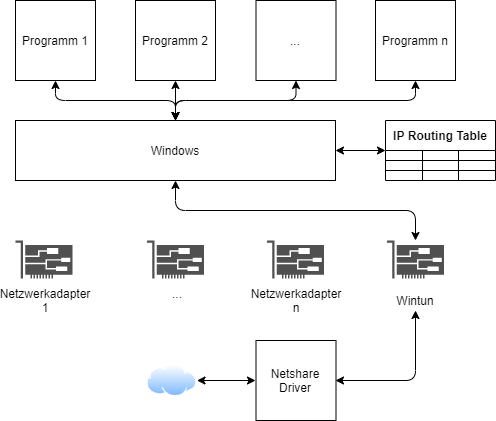
\includegraphics[width=0.8\textwidth]{diagramm_sammel_von_ip_paketen.png}
    \caption[Sammeln von IP Paketen]{Sammeln von IP Paketen \footnotemark[1]{Vgl. \ref{flasklogo}}} 
\end{figure}